\documentclass[10pt]{beamer}

\usetheme[progressbar=frametitle]{metropolis}
\usepackage{appendixnumberbeamer}
\usepackage{minted}
\usepackage{booktabs}
\usepackage[scale=2]{ccicons}

\usepackage{pgfplots}
\usepgfplotslibrary{dateplot}

\usepackage{xspace}
\newcommand{\themename}{\textbf{\textsc{metropolis}}\xspace}

\title{Clash - Haskell as an HDL}
\subtitle{A quick introduction}
% \date{\today}
\date{}
\author{Martijn Bastiaan <martijn@qbaylogic.com>}
\institute{
\includegraphics[height=1.2cm]{img/logo-fpga-innovation-crop.pdf}}
\titlegraphic{\hfill}

\begin{document}

\maketitle

%\begin{frame}{Table of contents}
%  \setbeamertemplate{section in toc}[sections numbered]
%  \tableofcontents[hideallsubsections]
%\end{frame}

\begin{frame}[fragile]{QBayLogic and Clash}
  \begin{itemize}
  		\item \textbf{Clash}: high-level synthesis using Haskell
		\item Started as a research project in 2009
        \begin{itemize}
        	\item at the University of Twente (the Netherlands)
        	\item 20+ publications since then
            \item Spawned many related research topics
        \end{itemize}
		\item \textbf{QBayLogic B.V.} founded in 2016
		\item I joined in 2017 as software engineer
	\end{itemize}
\end{frame}
\begin{frame}[fragile]{Clash}
  Clash $\approx$ Haskell without:

  \begin{itemize}
  	\item General recursion
    \item Types sized at runtime (e.g., lists)
    \begin{itemize}
    	\item Lack of lists is amortized by \textbf{vectors}
    \end{itemize}
  \end{itemize}
  
Clash offers:

\begin{itemize}
	\item Strong typing guarantees
    \item Very high-level features without typical overhead
\end{itemize}
\end{frame}

\begin{frame}[fragile]{Clash}
  In this presentation we're going to build a very small CPU..
  
  \begin{itemize}
  	\item .. with \emph{n} registers
  	\item .. operating on arbitrary \emph{number types}
    \item .. executing one instruction per cycle
  \end{itemize}
\end{frame}

\begin{frame}[fragile]{Clash}
\begin{center}
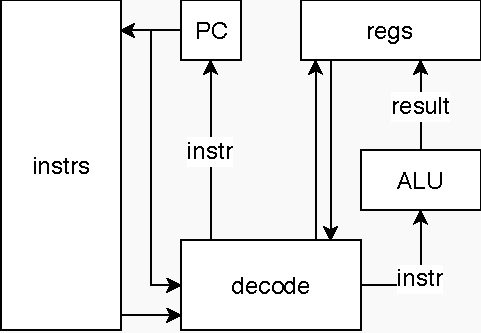
\includegraphics[width=0.8\textwidth]{img/CPU.pdf}
\end{center}
\end{frame}

\begin{frame}[fragile]{Clash}
\begin{center}
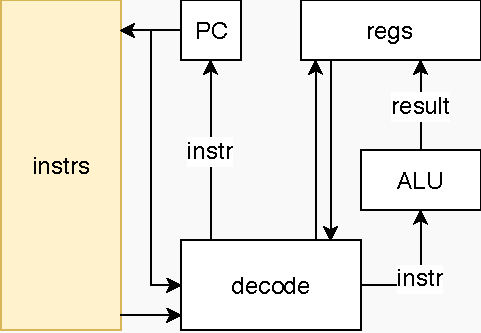
\includegraphics[width=0.8\textwidth]{img/CPU-instrs.pdf}
\end{center}
\end{frame}

\begin{frame}[fragile]{Instruction set}
\begin{minted}{haskell}
  data Instruction n numType
\end{minted}
\pause
\begin{minted}{haskell}
    = Multiply (Reg n) (Reg n) (Reg n)
\end{minted}
\pause
\begin{minted}{haskell}
    | Add      (Reg n) (Reg n) (Reg n)
\end{minted}
\pause
\begin{minted}{haskell}
    | Absolute (Reg n)         (Reg n)
\end{minted}
\pause
\begin{minted}{haskell}
    | Literal  numType         (Reg n)
\end{minted}
\pause
\begin{minted}{haskell}
    | Jump     Int8
\end{minted}
\pause

\begin{minted}{haskell}
  type Reg n = Index n
\end{minted}
\end{frame}

\begin{frame}[fragile]{Clash}
\begin{center}
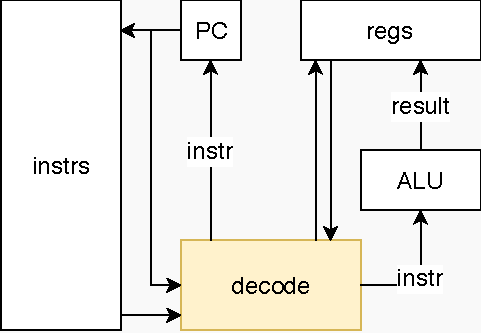
\includegraphics[width=0.8\textwidth]{img/CPU-decode.pdf}
\end{center}
\end{frame}

\begin{frame}[fragile]{Decoded instruction set}
Decoded ALU instructions are much simpler than the original instruction set:

  \begin{minted}{haskell}
  data ALUInstruction
    = Add' 
    | Multiply' 
    | Absolute'
  \end{minted}
\pause
  
Same goes for the the program counter instruction set:
  
  \begin{minted}{haskell}
  data PCInstruction
    = Jump' Int8
    | Succ
  \end{minted}
\end{frame}

\begin{frame}[fragile]{Decoder}
\begin{minted}{haskell}
decode regs (Add x y z) = 
  (Add', Succ, regs !! x, regs !! y, z)
\end{minted}

\pause

\begin{minted}{haskell}
decode regs (Multiply x y z) = 
  (Multiply', Succ, regs !! x, regs !! y, z)
\end{minted}

\pause

\begin{minted}{haskell}
decode regs (Absolute x z) = 
  (Absolute', Succ, regs !! x, undefined, z)
\end{minted}

\pause

\begin{minted}{haskell}
decode regs (Literal x z) = 
  (Add', Succ, x, 0, z)
\end{minted}

\pause

\begin{minted}{haskell}
decode regs (Jump z) = 
  (undefined, Jump' z, undefined, undefined, 0)
\end{minted}
\end{frame}


\begin{frame}[fragile]{Clash}
\begin{center}
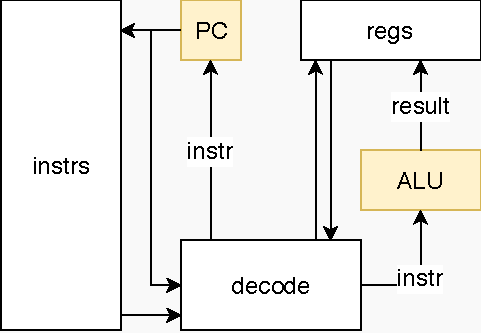
\includegraphics[width=0.8\textwidth]{img/CPU-ALU-PC.pdf}
\end{center}
\end{frame}

\begin{frame}[fragile]{ALU}
The ALU takes an ALU instruction and executes it:

  \begin{minted}{haskell}
  alu Add'      x y = x + y
  alu Multiply' x y = x * y
  alu Absolute' x _ = abs x
  \end{minted}
  
\pause
  
And the program counter does the same:

  \begin{minted}{haskell}
  nextPC pc  Succ     = pc + 1
  nextPC _  (Jump' n) = n
  \end{minted}
\end{frame}

\begin{frame}[fragile]{Clash}
\begin{center}
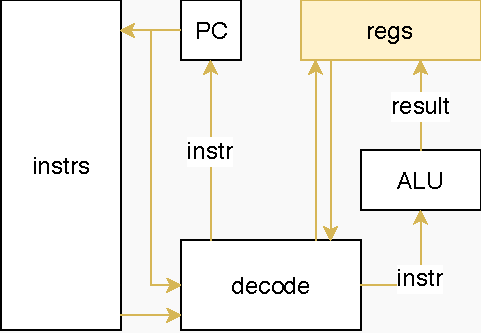
\includegraphics[width=0.8\textwidth]{img/CPU-misc.pdf}
\end{center}
\end{frame}

\begin{frame}[fragile]{Processor}
  \begin{minted}{haskell}
proc instrs (regs, pc) _ = ((regs'', pc'), result)
  where
\end{minted}
  \pause
\begin{minted}{haskell}    
    (aluInstruction, pcInstruction, x, y, wrAddr) = 
      decode regs (instrs !! pc)
  \end{minted}
\pause
  \begin{minted}{haskell}
    result = alu aluInstruction x y
  \end{minted}
  \pause
  \begin{minted}{haskell}
    regs'  = replace wrAddr result regs
    regs'' = replace 0      0      regs'
  \end{minted}
  \pause
  \begin{minted}{haskell}
    pc' = nextPC pc pcInstruction
  \end{minted}
\end{frame}

\section{Simulation}

\begin{frame}[fragile]{Simulation: 16 bits}
  \begin{minted}{haskell}
instrs :: Vec 4 (Instruction 3 Int16)
instrs = Literal 5 1
      :> Literal 7 2
      :> Add 1 2 1
      :> Jump 2
      :> Nil
  
regs :: Vec 3 Int16
regs = 0 :> 0 :> 0 :> Nil
  
results =
  mealy (proc instrs) regs (pure ())
  \end{minted}
\end{frame}

\begin{frame}[fragile]{Simulation: 16 bits}
\begin{verbatim}
$ clashi Proc.hs 
*Proc> showX $ sampleN 8 results
[5, 7, 12, X, 19, X, 26, X]
\end{verbatim}
\end{frame}

\begin{frame}[fragile]{Simulation: vectors}
\begin{minted}{haskell}
instance (KnownNat n, Num a) => Num (Vec n a) where
  (+) = zipWith (+)
  (*) = zipWith (*)
  (-) = zipWith (-)
  abs = map abs
\end{minted}
\end{frame}

\begin{frame}[fragile]{Simulation: vectors}
  \begin{minted}{haskell}
instrsVec :: Vec 4 (Instruction 3 (Vec 2 Int16))
instrsVec 
  = Literal (5 :> 6 :> Nil) 1
 :> Literal (7 :> 8 :> Nil) 2
 :> Add 1 2 1
 :> Jump 2
 :> Nil
  
regsVec :: Vec 3 (Vec 2 Int16)
regsVec = repeat (0 :> 0 :> Nil)
  
resultsVec =
  mealy (proc instrs) regs (pure ())
  \end{minted}
\end{frame}

\begin{frame}[fragile]{Simulation: vectors}
\begin{verbatim}
$ clashi Proc.hs 
*Proc> showX $ sampleN 8 resultsVec
[<5,6>, <7,8>, <12,14>, X, <19,22>, X, <26,30>, X]
\end{verbatim}
\end{frame}

\begin{frame}[fragile]{Simulation: matrices}
\begin{minted}{haskell}
-- | Dot product on vectors
dot as bs = sum $ zipWith (*) as bs
\end{minted}

\begin{minted}{haskell}
-- | Matrix is a 2D "array"
type Matrix m n a = Vec m (Vec n a)
\end{minted}

\begin{minted}{haskell}
-- | Num instance for matrices
instance (.., Num a) => Num (Matrix m n a) where
  (+) = zipWith (+)
  (-) = zipWith (-)
  a*b = transpose (zipWith dot a (transpose b))
  abs = map abs
\end{minted}
\end{frame}

\begin{frame}[fragile]{Conclusion}

We've built a small CPU that handles

\begin{itemize}
\item Integers, floats, vectors, ..
\item .. any other ``Num instances''
\end{itemize}

\pause

We've used our own datatypes to:

\begin{itemize}
\item define an internal instruction set
\item \emph{use} that IS as an assembly-type language in simulation
\end{itemize}

\end{frame}

\begin{frame}[fragile]
\vfill

\begin{center}
{\Huge Q\&A}
\end{center}

\vfill

\begin{center}

\includegraphics[width=0.6\textwidth]{img/logo-fpga-innovation-crop.pdf} \\
Martijn Bastiaan <martijn@qbaylogic.com> \\
http://clash-lang.org/ 
\end{center}
\end{frame}

\end{document}
